% ==============================================================================
% 04_capteurs_donnees.tex - Module 4 (15h30 - 16h30)
% Exemple de capteurs et mesures spécifiques : de la collecte à la donnée
% Pratique : Ping Sonar, Ping360, DVL-A50, intégration d'une sonde scientifique tierce
% ==============================================================================

\section{Module 4 : Capteurs Pratiques \& Chaîne de Traitement de Données}

\begin{frame}{4.1 Typologie : Capteurs de Sûreté vs Recueil de Données}
  \begin{columns}[T]
    \begin{column}{0.49\textwidth}
      \begin{alertblock}{1. Capteurs de Sûreté Véhicule (Vital)}
        \scriptsize
        \textit{Assurent la survie et l'intégrité matérielle du robot :}
        \begin{itemize}
          \item \alertw{SOS Leak Sensors} : rubans conductimétriques au point le plus bas de chaque caisson étanche $\rightarrow$ alerte MAVLink immédiate, arrêt propulsion, remontée passive.
          \item \textbf{Pression/Température interne (Bar02)} : surveillance active du vide résiduel post-vacuum test $\rightarrow$ alerte d'infiltration avant tout contact liquide.
          \item \textbf{Power Sense (Courant/Tension)} : surveillance en temps réel de l'état des cellules Li-ion et consommation des propulseurs.
        \end{itemize}
      \end{alertblock}
    \end{column}

    \begin{column}{0.49\textwidth}
      \begin{exampleblock}{2. Capteurs \& Indicateurs de Données}
        \scriptsize
        \textit{Charge utile scientifique dédiée à la mission :}
        \begin{itemize}
          \item \textbf{Optique \& Éclairage} : \succw{caméras étanches Low-Light HD/4K}, \succw{projecteurs Lumen ($1500\text{--}6000\,\text{lm}$)}, \succw{lasers de dimensionnement}.
          \item \textbf{Acoustique \& Relief} : Ping Sonar, Ping360, Omniscan 2D, MBES multifaisceaux bathymétrique.
          \item \textbf{Odométrie \& Positionnement} : DVL-A50 (effet Doppler), antenne USBL de surface.
          \item \textbf{Physico-chimie de l'eau} : sonde CTD (salinité, masse volumique, célérité), fluorimètre, $\text{O}_2$ dissous.
        \end{itemize}
      \end{exampleblock}
    \end{column}
  \end{columns}
\end{frame}

\begin{frame}{4.0b Caméras Sous-Marines : Low-Light HD vs Nouvelle 4K Cam}
  \begin{columns}[T]
    \begin{column}{0.48\textwidth}
      \begin{center}
        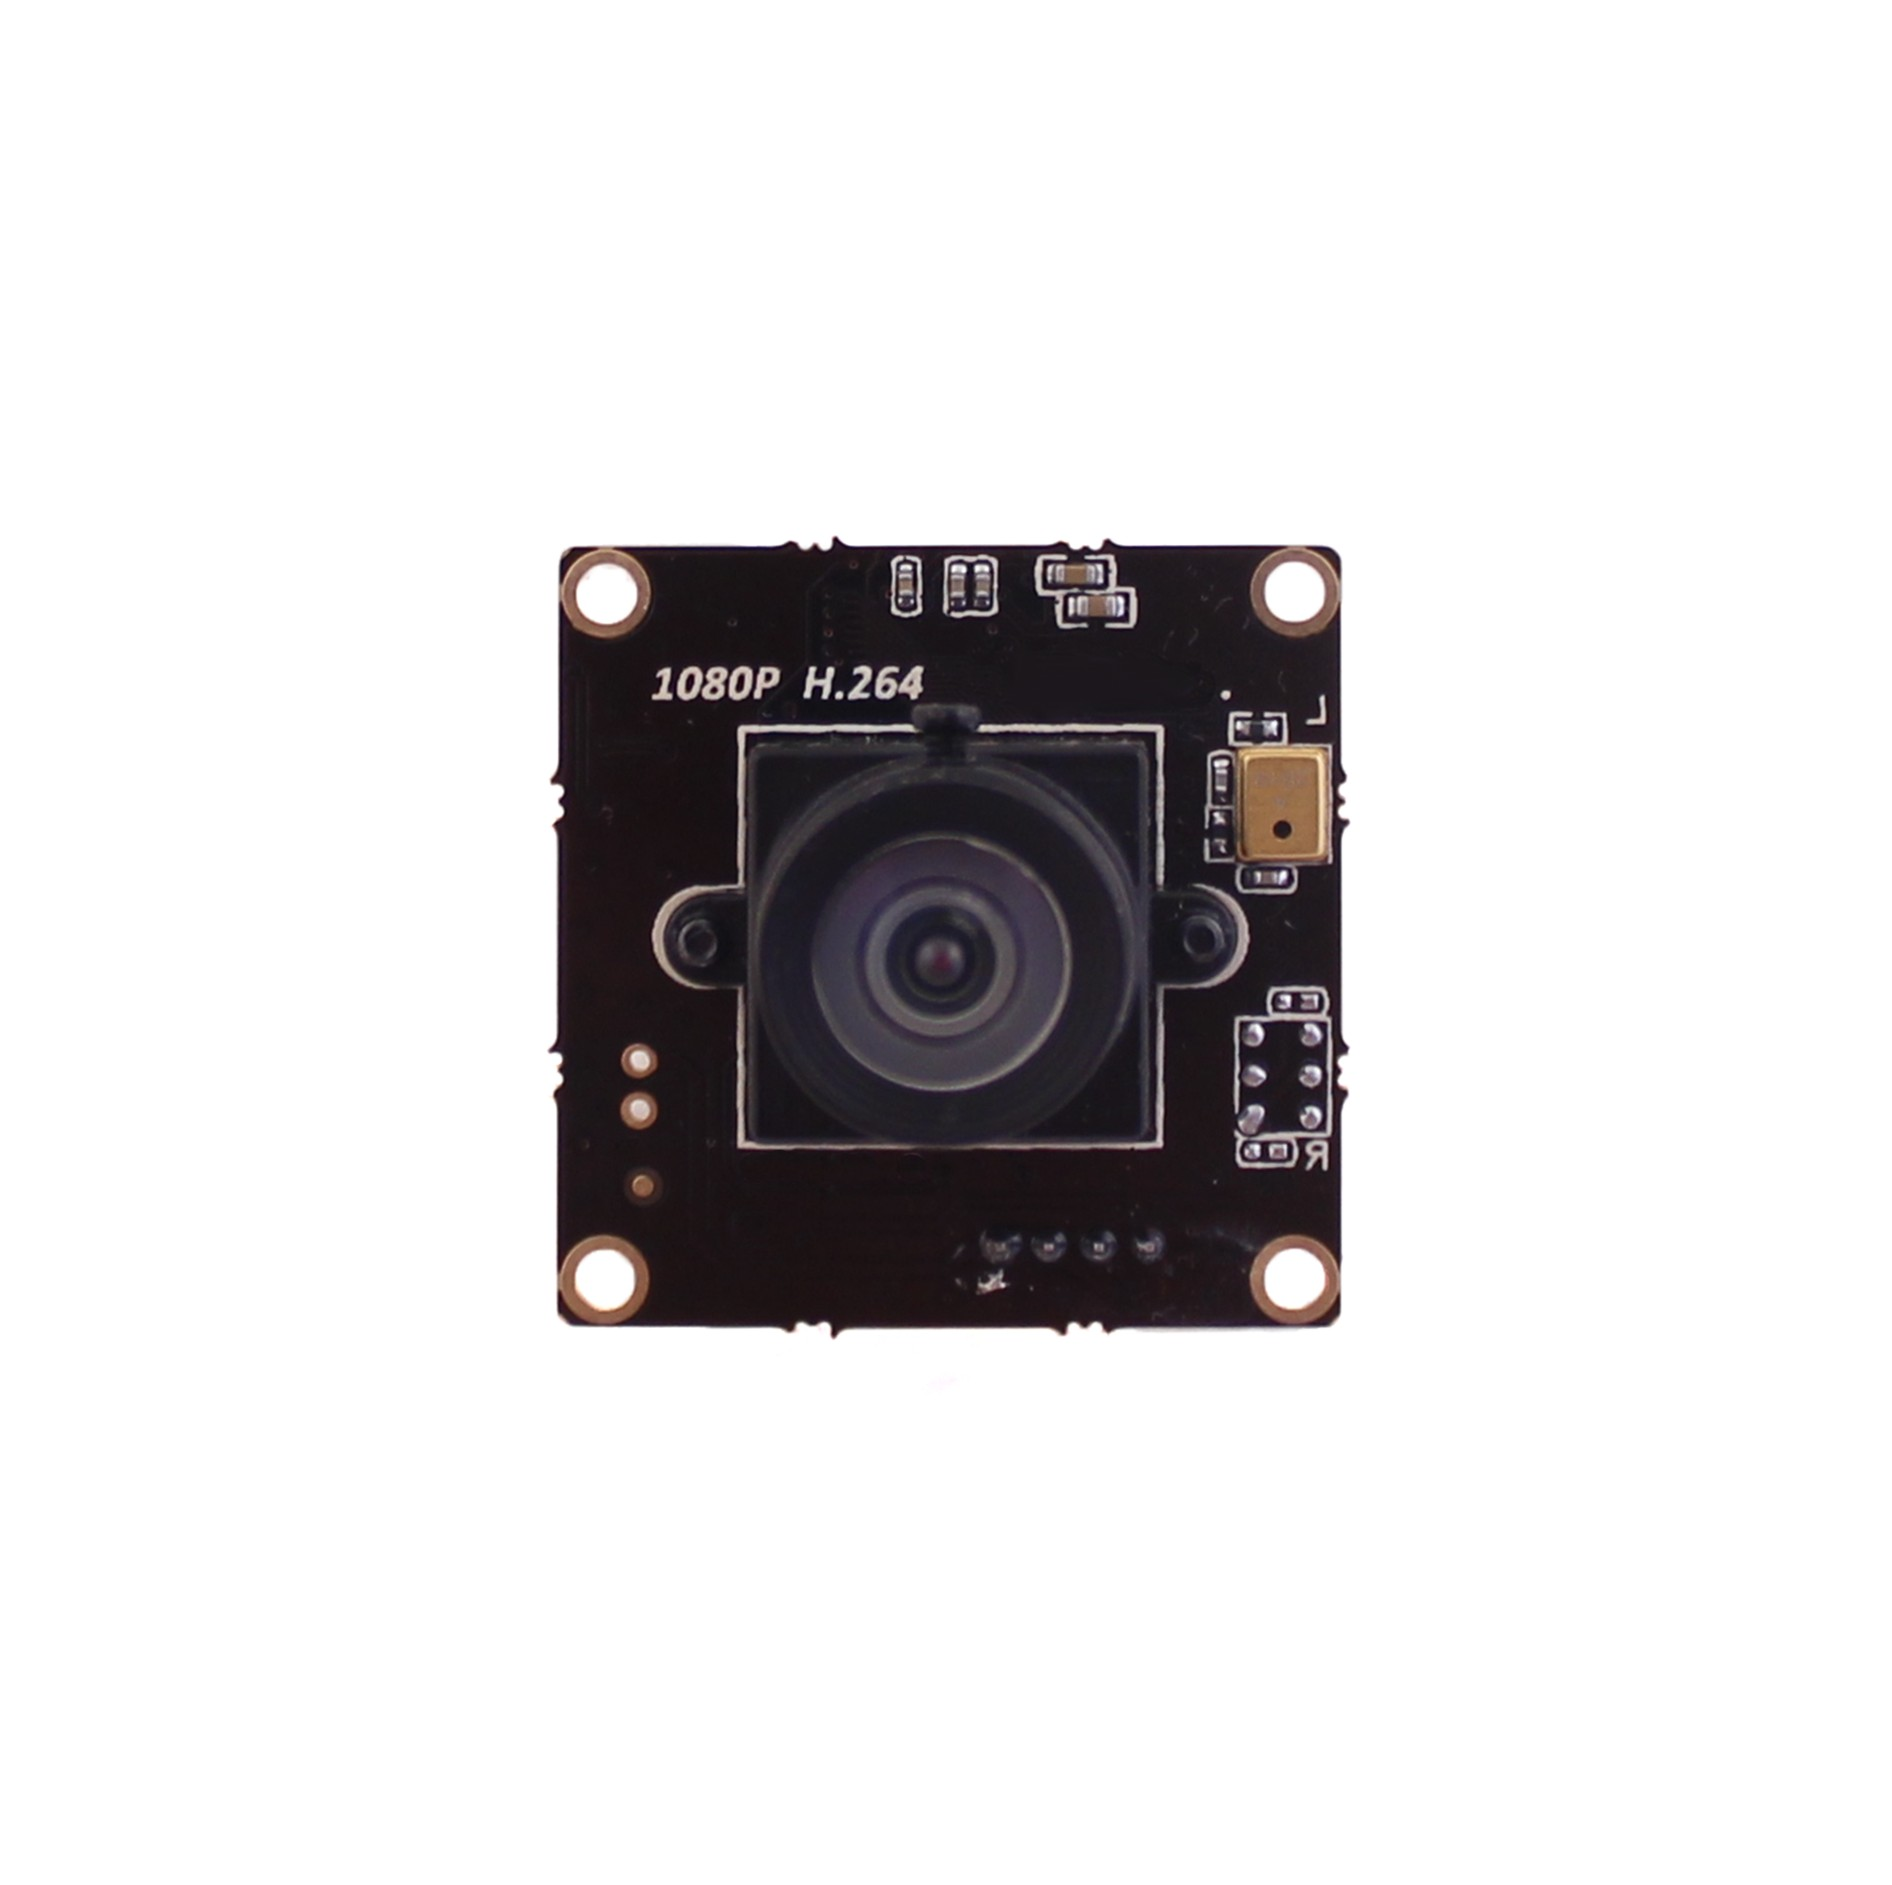
\includegraphics[height=2.2cm, keepaspectratio]{camera_hd.jpg}\\
        \vspace{0.2em}
        \tech{Caméra Low-Light HD (Standard)}\\
        \tiny\textit{Capteur Sony CMOS $\cdot$ $1080\text{p}@30\,\text{fps}$ $\cdot$ $0.01\,\text{lux}$}
      \end{center}
      \scriptsize
      \begin{itemize}
        \item \textbf{Standard BlueROV2} : caméra USB compacte montée sur berceau pivotant commandé par servomoteur PWM.
        \item \textbf{Nacelle tilt motorisée} : orientable de $+45^\circ$ (navigation avant) à $-90^\circ$ (vue benthique au nadir).
        \item \textbf{Basse latence} : flux H.264 temps réel $<120\,\text{ms}$ vers QGroundControl / Cockpit.
        \item Dôme acrylique hémisphérique corrigeant la réfraction.
      \end{itemize}
    \end{column}

    \begin{column}{0.48\textwidth}
      \begin{center}
        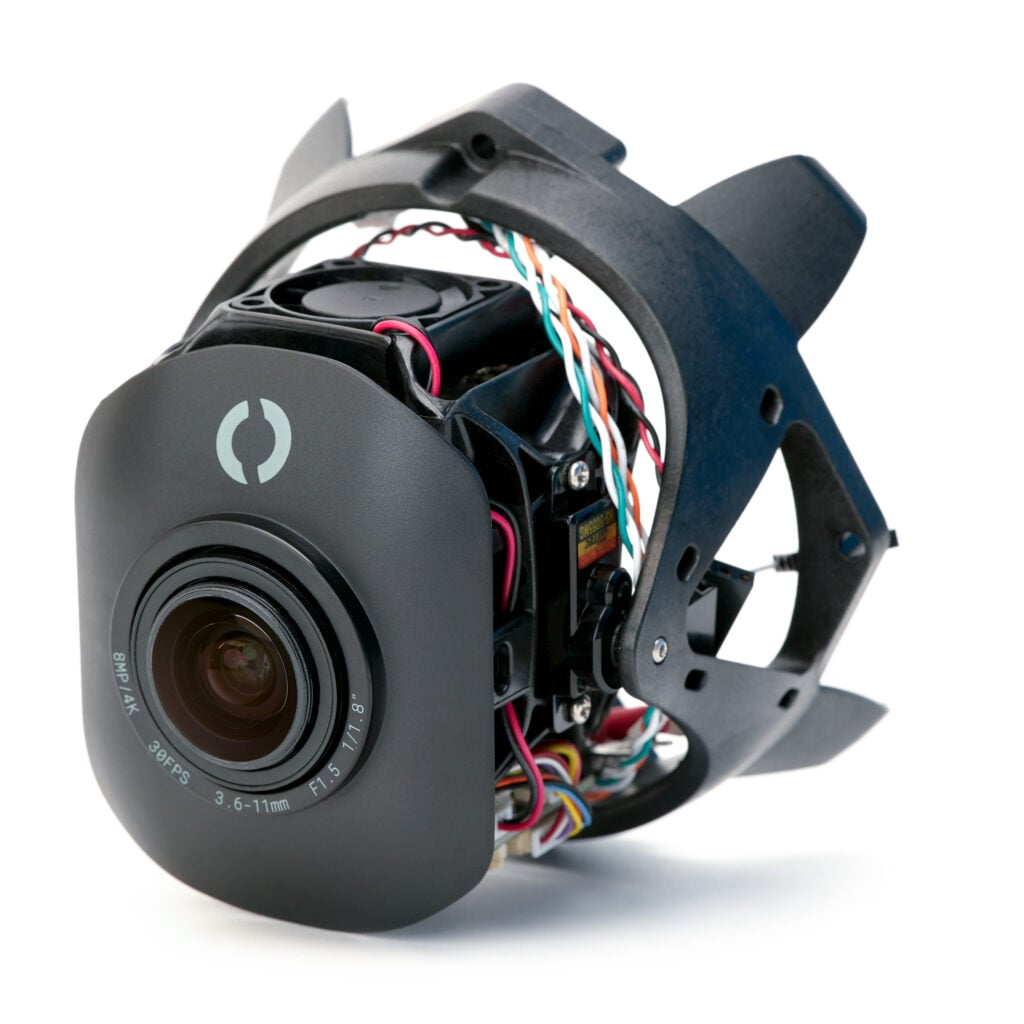
\includegraphics[height=2.2cm, keepaspectratio]{camera_4k.jpg}\\
        \vspace{0.2em}
        \succw{Nouvelle 4K Cam (Ultra-HD \& Zoom)}\\
        \tiny\textit{Capteur Sony Starvis 2 IMX678 $\cdot$ $4\text{K} \ (3840\times 2160)$ $\cdot$ $0.001\,\text{lux}$}
      \end{center}
      \scriptsize
      \begin{itemize}
        \item \textbf{Haute Résolution \& Détails} : $4\times$ plus de pixels pour l'identification taxonomique et la photogrammétrie fine.
        \item \textbf{Optique motorisée} : autofocus rapide et zoom numérique/optique pilotable en direct depuis l'interface Cockpit.
        \item \textbf{Sensibilité extrême} : capteur Starvis 2 rétroéclairé pour les plongées profondes et zones sombres.
        \item Rétrocompatible avec le dôme 4" du BlueROV2.
      \end{itemize}
    \end{column}
  \end{columns}
\end{frame}

\begin{frame}{4.0c Éclairage Étanche \& Échelle : Feux Lumen \& Lasers}
  \begin{columns}[T]
    \begin{column}{0.48\textwidth}
      \begin{center}
        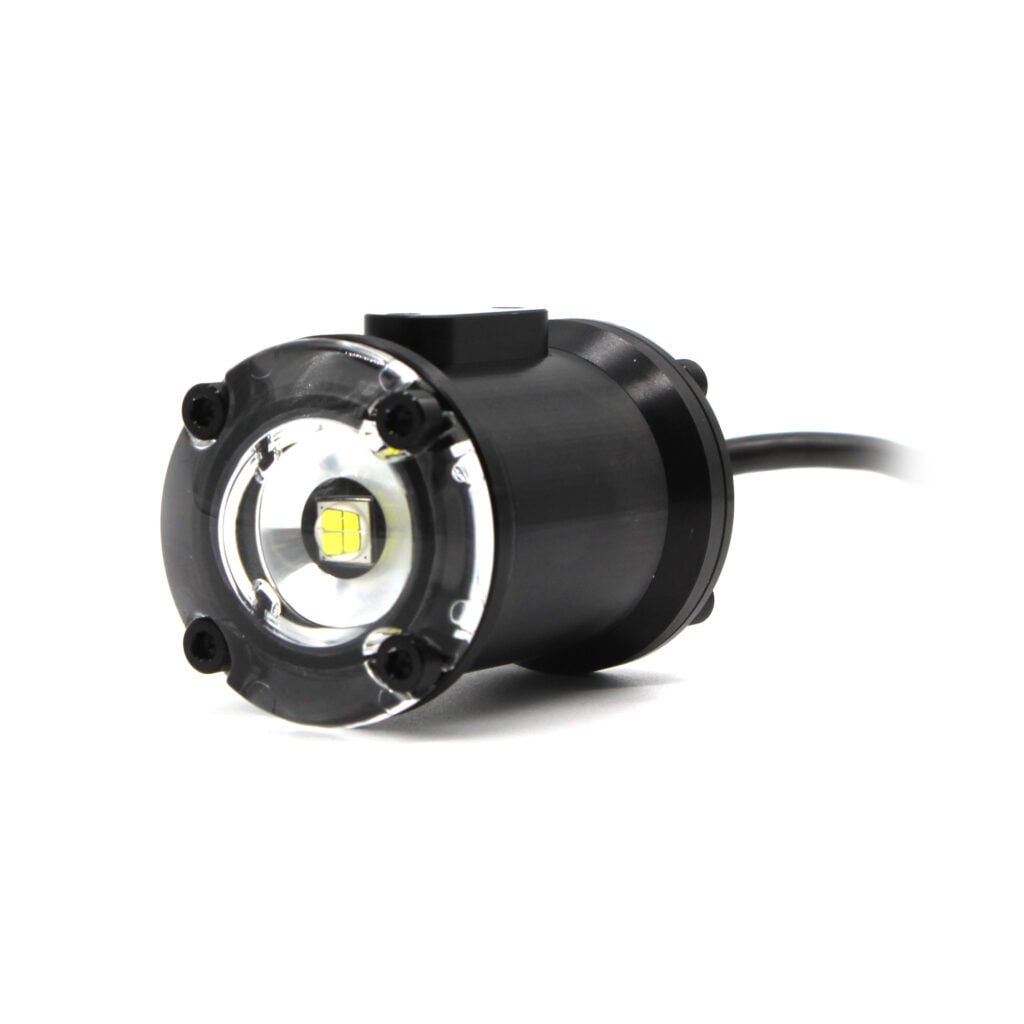
\includegraphics[height=2.2cm, keepaspectratio]{lumen_light.jpg}\\
        \vspace{0.2em}
        \tech{Projecteur Lumen Subsea Light}\\
        \tiny\textit{LED haute puissance $\cdot$ $1500\text{--}6000\,\text{lm}$ $\cdot$ Étanche $500\,\text{m}$ (50 bar)}
      \end{center}
      \scriptsize
      \begin{itemize}
        \item \textbf{Restauration chromatique} : compense la disparition rapide du spectre rouge dès $3\text{--}5\,\text{m}$ de profondeur.
        \item \textbf{Montage déporté vital} : espacé des caméras pour supprimer la rétrodiffusion (*backscatter*) sur la neige marine.
        \item \textbf{Pilotage PWM fin} : intensité variable depuis la manette pour éviter d'éblouir la faune ou saturer l'image.
        \item Balise stroboscopique de repérage en surface.
      \end{itemize}
    \end{column}

    \begin{column}{0.48\textwidth}
      \begin{center}
        \begin{tikzpicture}[scale=0.78]
          % Fond marin
          \draw[thick, fill=brown!20] (-2.2, -1.2) rectangle (2.2, -0.6);
          \node at (0, -0.9) {\tiny Fond benthique / Faune};
          % Cible
          \draw[thick, fill=OceanGreen!40] (-0.8, -0.6) rectangle (0.8, -0.3);
          \node at (0, -0.45) {\tiny Spécimen biologique ($10\,\text{cm}$)};
          % Points laser
          \fill[green!80!black] (-0.5, -0.3) circle (3pt);
          \fill[green!80!black] (0.5, -0.3) circle (3pt);
          \draw[<->, thick, green!70!black] (-0.5, 0.0) -- (0.5, 0.0) node[midway, above] {\tiny $\Delta x = 100\,\text{mm}$ calibré};
          % Faisceaux
          \draw[dashed, green!80!black, line width=1.2pt] (-0.5, 1.4) -- (-0.5, -0.3);
          \draw[dashed, green!80!black, line width=1.2pt] (0.5, 1.4) -- (0.5, -0.3);
          % Boîtier laser
          \draw[thick, fill=OceanDeep!80] (-0.9, 1.4) rectangle (-0.1, 1.8);
          \draw[thick, fill=OceanDeep!80] (0.1, 1.4) rectangle (0.9, 1.8);
          \node[white] at (-0.5, 1.6) {\tiny Laser 1};
          \node[white] at (0.5, 1.6) {\tiny Laser 2};
        \end{tikzpicture}\\
        \vspace{0.2em}
        \alertw{Lasers de Dimensionnement Sous-Marins}\\
        \tiny\textit{Double faisceau vert parallèle $\cdot$ Référence métrique absolue}
      \end{center}
      \scriptsize
      \begin{itemize}
        \item Deux lasers étanches montés à distance rigoureusement fixe ($50$ ou $100\,\text{mm}$).
        \item Projettent 2 points d'échelle métrique directe sans contact sur les captures vidéo (biométrie, géologie).
      \end{itemize}
    \end{column}
  \end{columns}
\end{frame}

\begin{frame}{4.1 Les Sonars Concrets du Chercheur : Ping Sonar \& Ping360}
  \begin{columns}[T]
    \begin{column}{0.48\textwidth}
      \begin{center}
        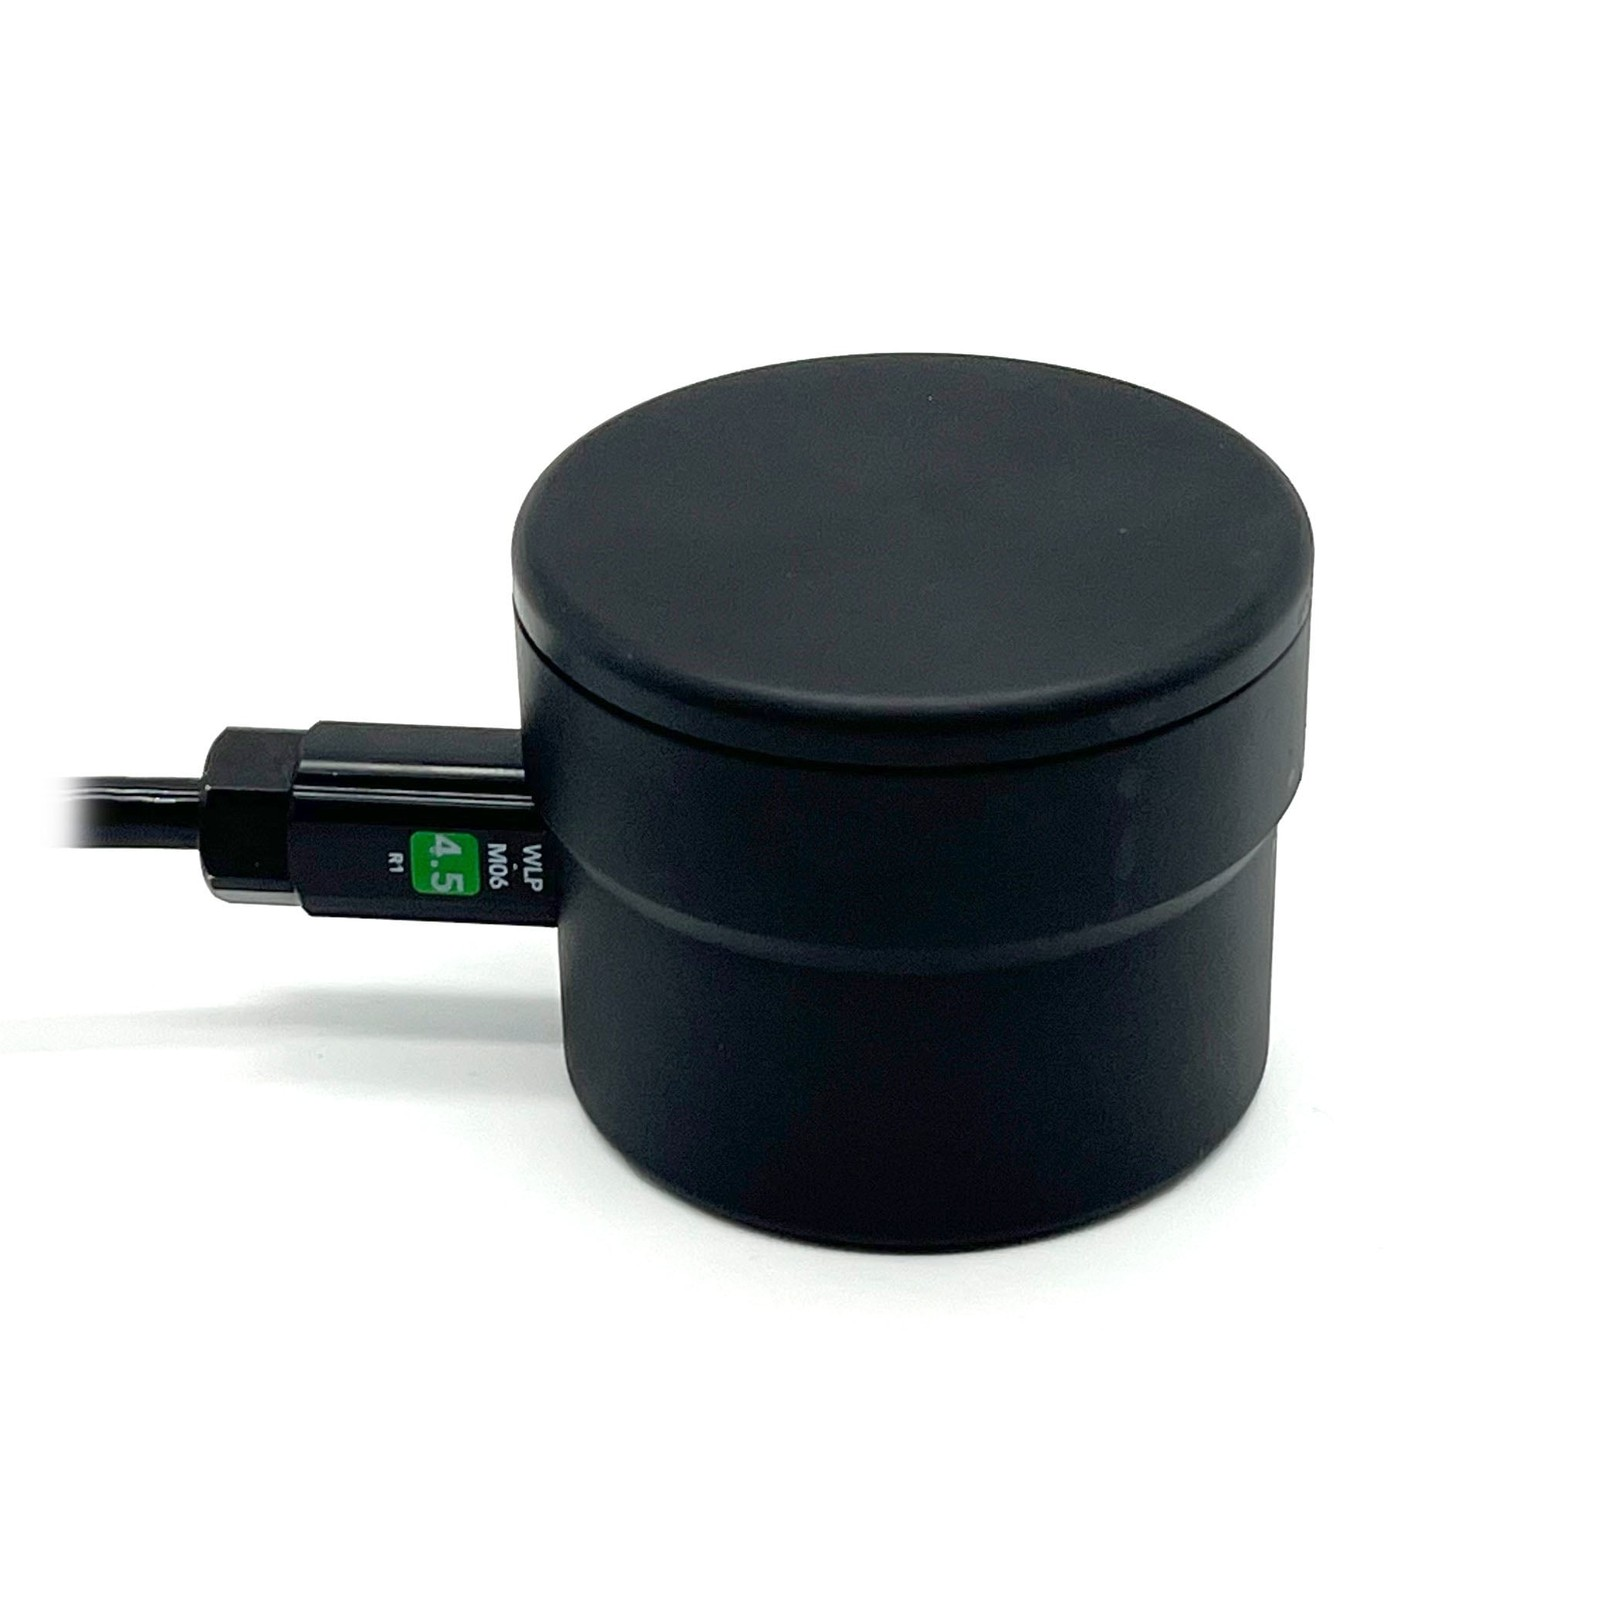
\includegraphics[height=2.3cm, keepaspectratio]{ping_echosounder.jpg}\\
        \vspace{0.2em}
        \tech{Ping Sonar (Échosondeur 115 kHz)}
      \end{center}
      \scriptsize
      \begin{itemize}
        \item \textbf{Principe} : mono-faisceau vertical ($30^\circ$).
        \item Portée : $0.5\,\text{m}$ à $50\,\text{m}$.
        \item Interface : série UART / USB ($115200\,\text{bauds}$).
        \item \textbf{Usages} : altimètre pour \textit{bottom-following} sur ROV et bathymétrie simple sur BlueBoat.
        \item Librairie Python ouverte : \code{ping-python}.
      \end{itemize}
    \end{column}

    \begin{column}{0.48\textwidth}
      \begin{center}
        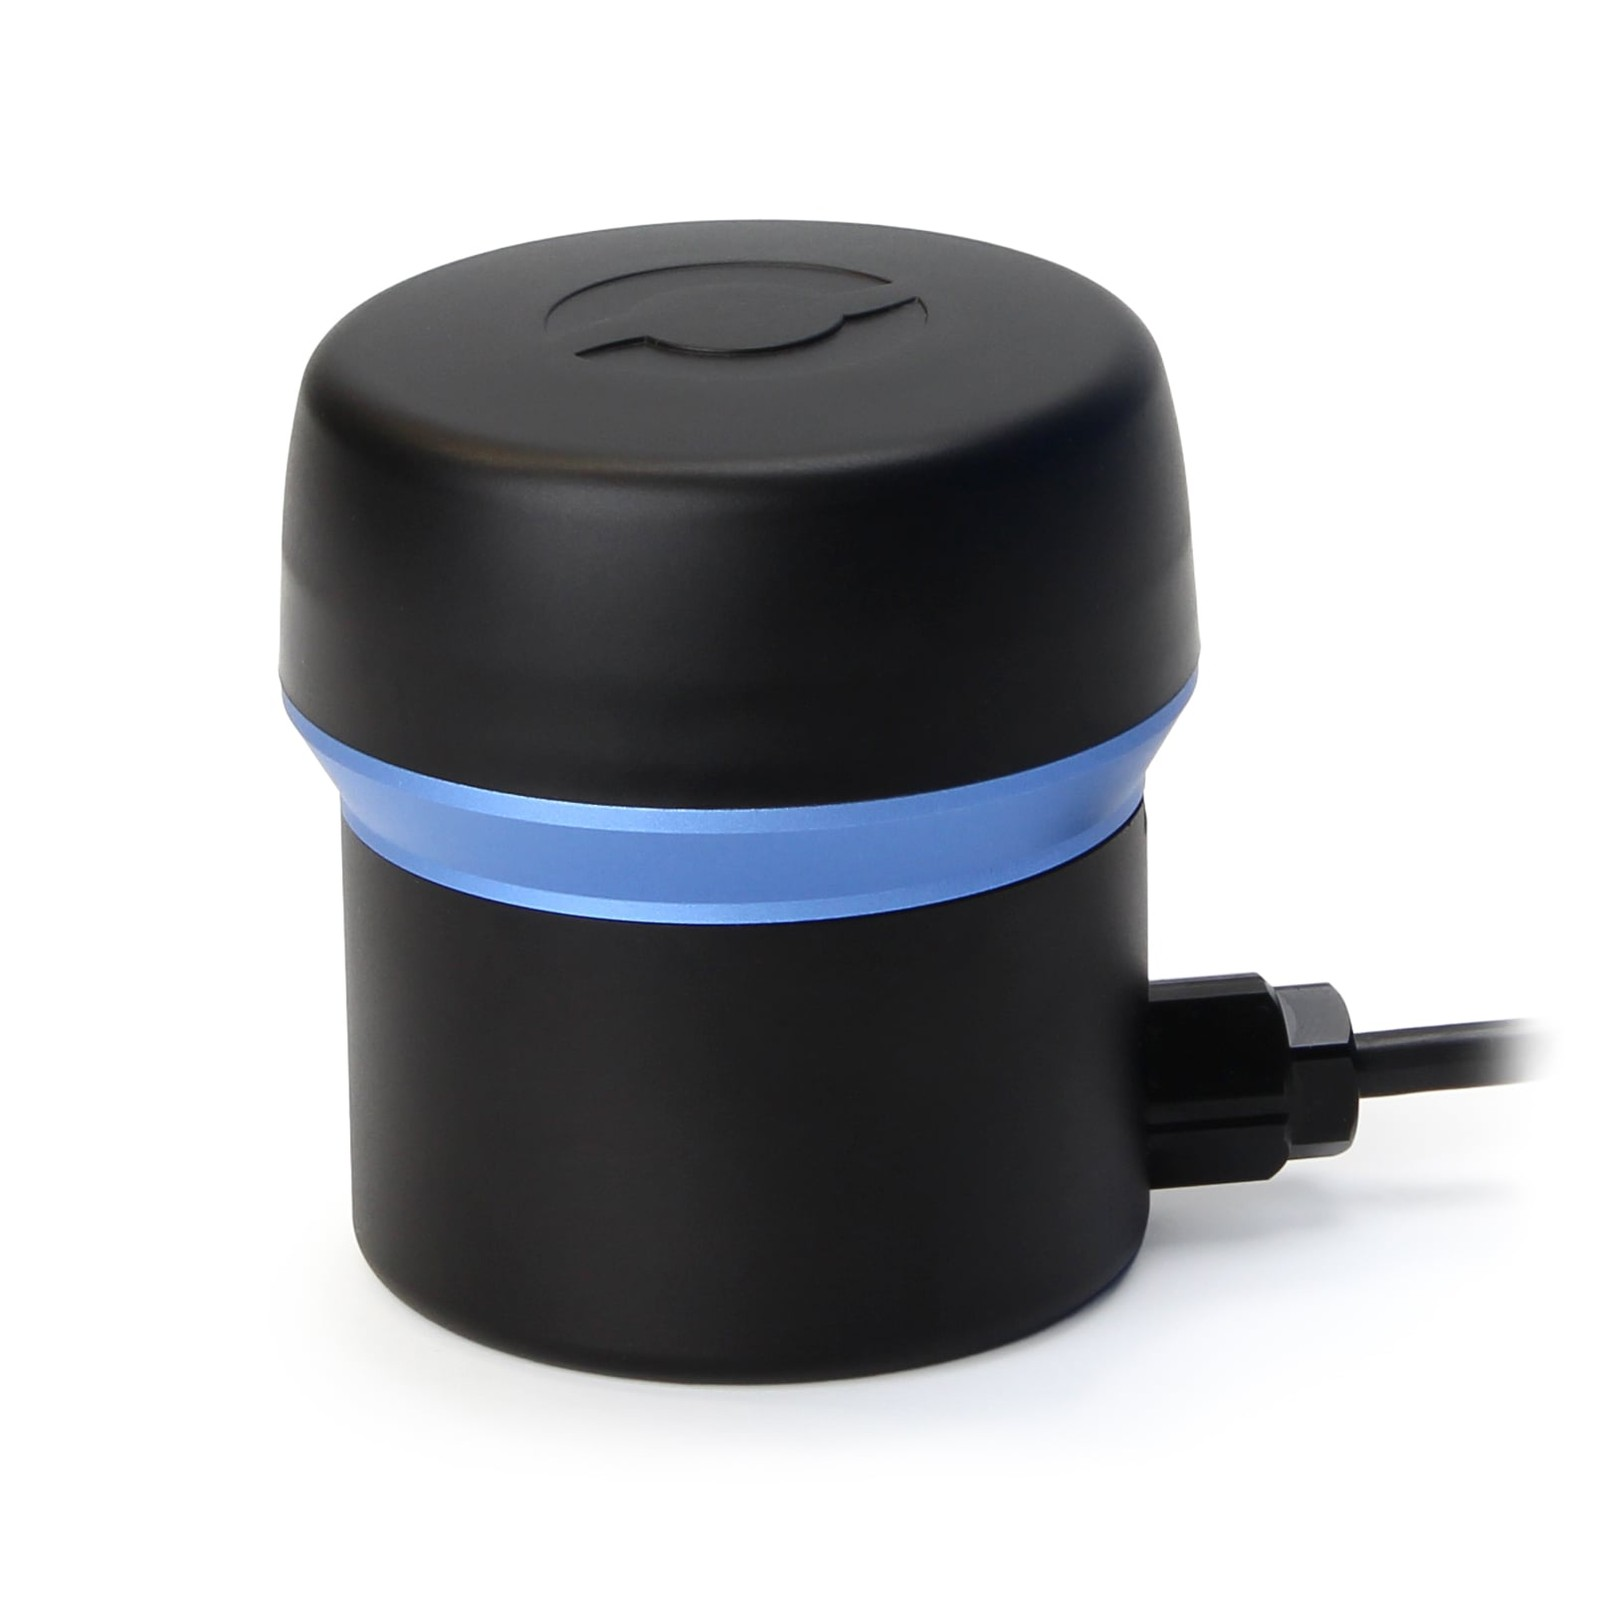
\includegraphics[height=2.3cm, keepaspectratio]{ping360_sonar.jpg}\\
        \vspace{0.2em}
        \tech{Ping360 (Sonar à Balayage 750 kHz)}
      \end{center}
      \scriptsize
      \begin{itemize}
        \item \textbf{Principe} : transducteur piézo rotatif motorisé.
        \item Faisceau fin : $2^\circ$ horizontal $\times 30^\circ$ vertical.
        \item Portée : jusqu'à $50\,\text{m}$ de rayon.
        \item \textbf{Usages} : navigation et évitement d'obstacles en eau turbide, détection de falaises et épaves.
      \end{itemize}
    \end{column}
  \end{columns}
\end{frame}

\begin{frame}{4.1b Imagerie Acoustique \& Sondeur Multifaisceaux (MBES)}
  \begin{columns}[T]
    \begin{column}{0.48\textwidth}
      \begin{center}
        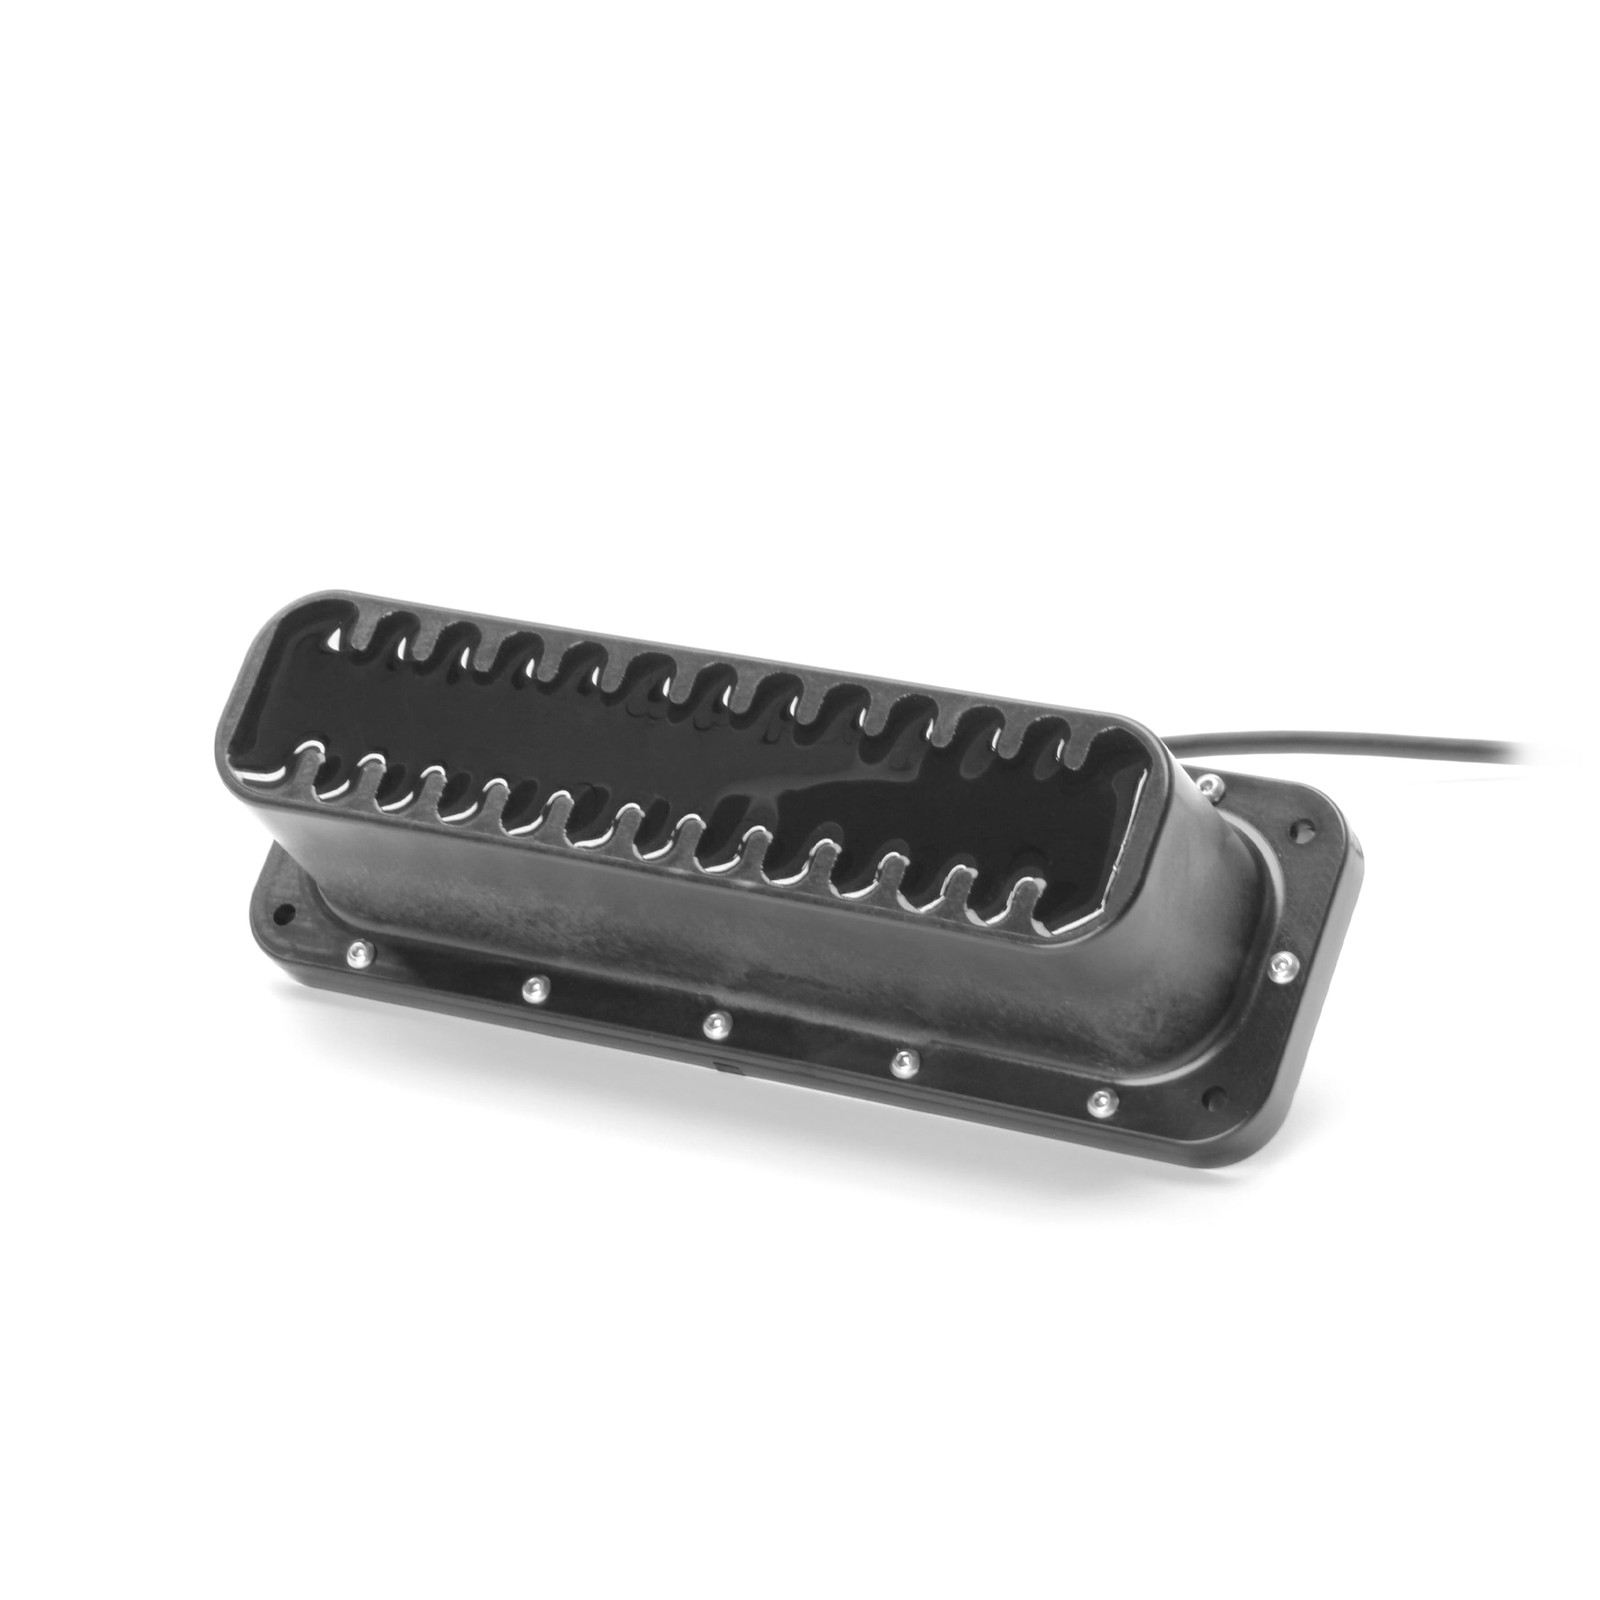
\includegraphics[height=2.4cm, keepaspectratio]{cerulean_omniscan.jpg}\\
        \vspace{0.2em}
        \tech{Cerulean Omniscan 450 FS}\\
        \footnotesize\textbf{Sonar d'Imagerie \& Balayage Avant}
      \end{center}
      \scriptsize
      \begin{itemize}
        \item \textbf{Fréquence} : $450\,\text{kHz}$, portée jusqu'à $100\,\text{m}$.
        \item \textbf{Imagerie acoustique 2D temps réel} : restitution d'échos haute résolution type "caméra acoustique".
        \item \textbf{Applications} : navigation en zéro visibilité, détection d'obstacles et cartographie latérale.
        \item Intégration directe BlueOS \& logiciel \textbf{SonarView}.
      \end{itemize}
    \end{column}

    \begin{column}{0.48\textwidth}
      \begin{center}
        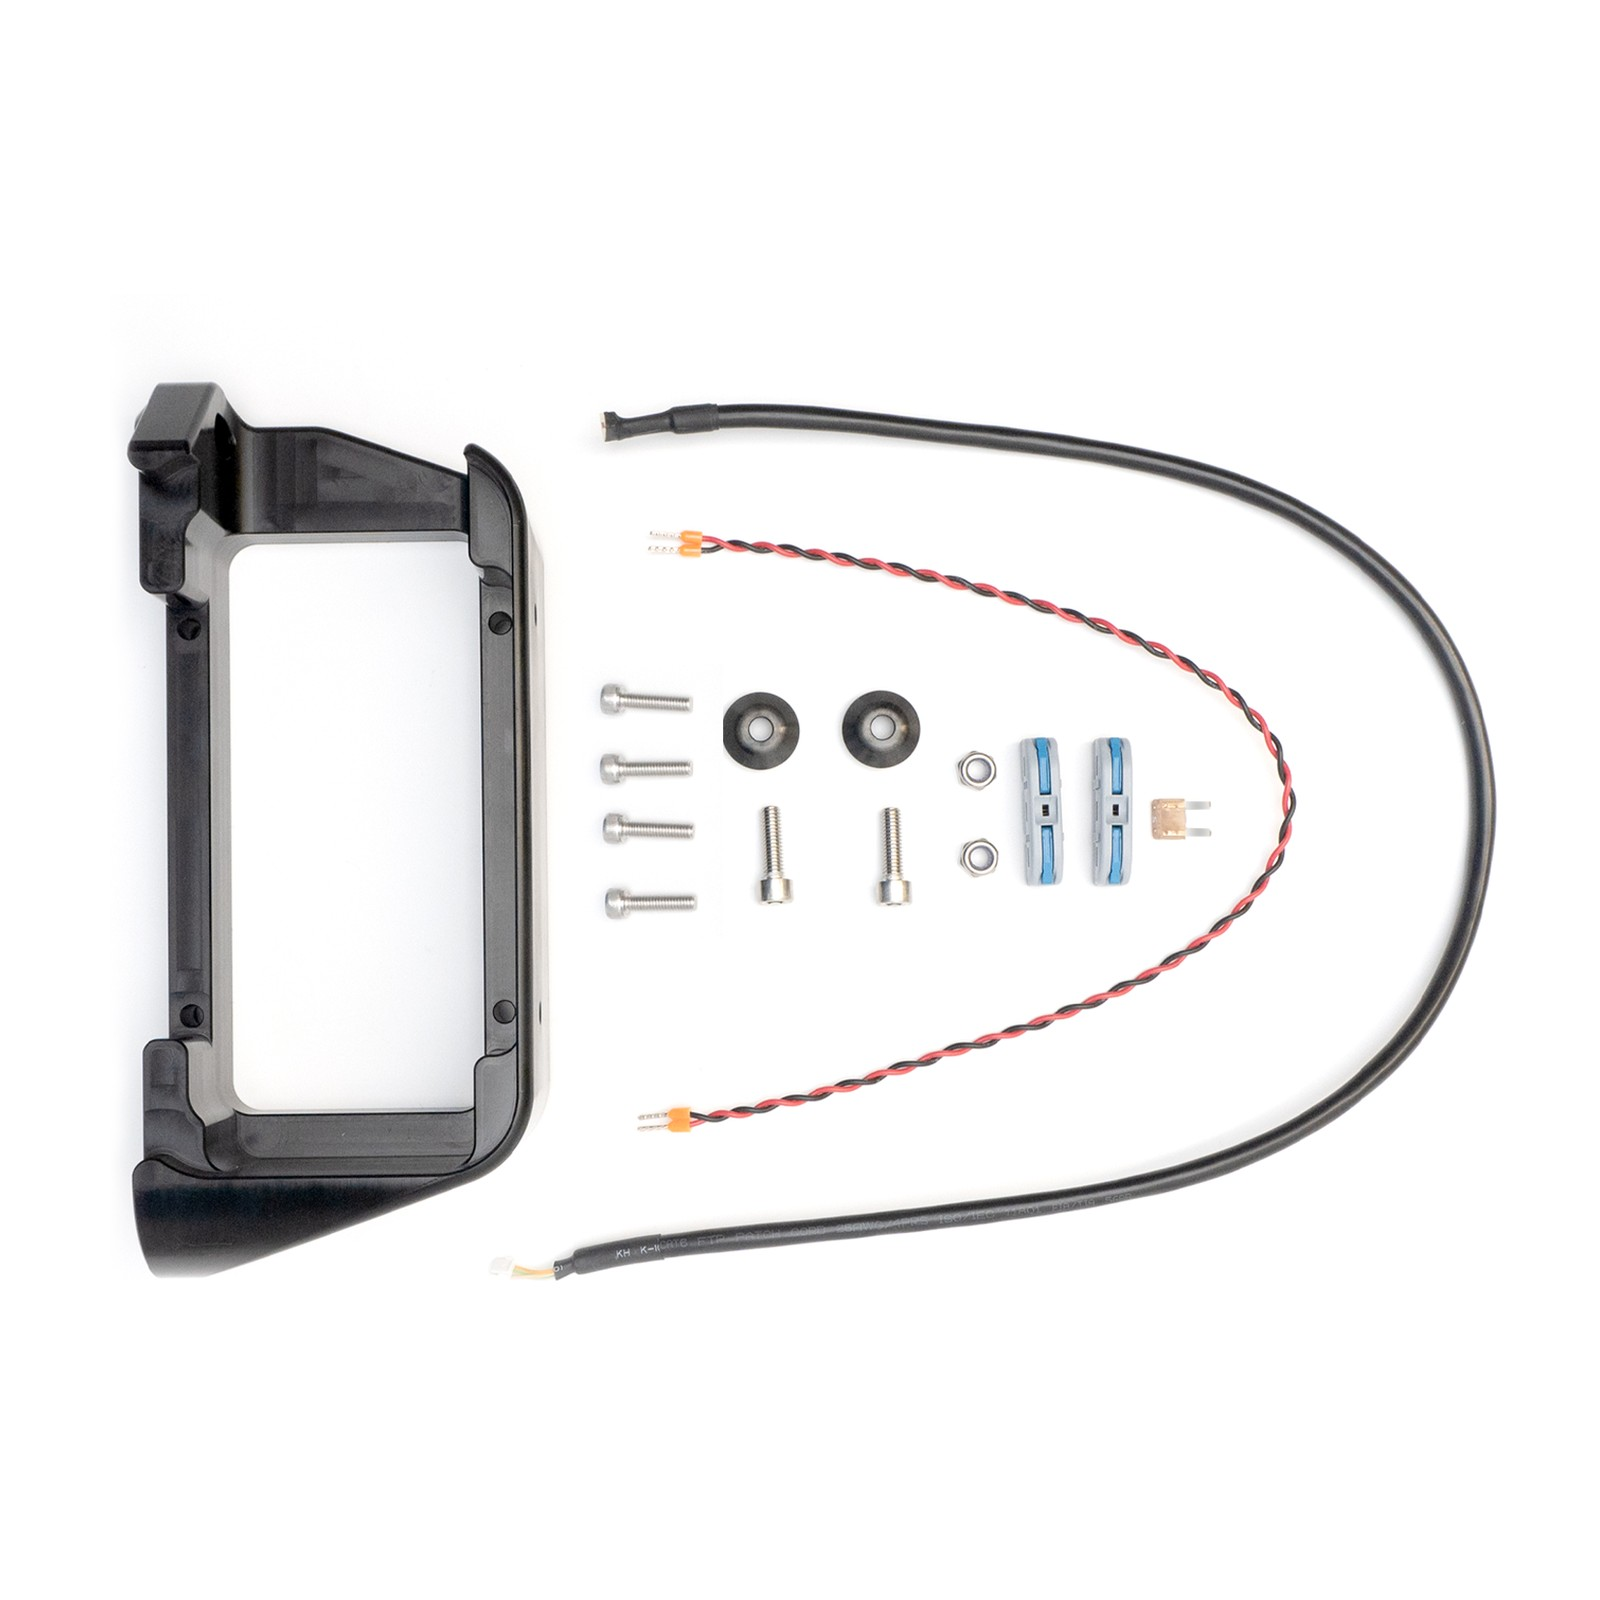
\includegraphics[height=2.4cm, keepaspectratio]{cerulean_surveyor_mbes.jpg}\\
        \vspace{0.2em}
        \tech{Cerulean Surveyor 240-16}\\
        \footnotesize\textbf{Multibeam Echosounder (MBES)}
      \end{center}
      \scriptsize
      \begin{itemize}
        \item \textbf{Multifaisceaux bathymétrique} : $240\,\text{kHz}$, 16 éléments de réception formés numériquement.
        \item \textbf{Fauchée 3D large} : cartographie bathymétrique surfacique (*swath*) haute densité sur \textbf{BlueBoat}.
        \item \textbf{Données denses} : nuages de points 3D couplés au GNSS RTK Centipede.
        \item Démocratisation des levés bathymétriques de laboratoire.
      \end{itemize}
    \end{column}
  \end{columns}
\end{frame}

\begin{frame}{4.2 Le DVL Embarqué : Water Linked DVL-A50}
  \begin{columns}[c]
    \begin{column}{0.54\textwidth}
      \textbf{La démocratisation de l'odométrie sous-marine} :
      \scriptsize
      \begin{itemize}
        \item Le \tech{Water Linked DVL-A50} :
          \begin{itemize}
            \item Poids dans l'eau : seulement \textbf{$270\,\text{g}$} (historiquement $>10\,\text{kg}$).
            \item 4 faisceaux Janus acoustiques à $1\,\text{MHz}$.
            \item Vitesse sol ($0.05\,\text{m}$ à $50\,\text{m}$ d'altitude fond).
          \end{itemize}
        \item \succw{Intégration directe BlueOS / ArduSub} :
          \begin{itemize}
            \item Se branche en Ethernet ou série sur le Raspberry Pi.
            \item Extension BlueOS dédiée disponible en 1 clic.
            \item Active le mode \textbf{Position Hold} : maintien stationnaire automatique face au courant.
          \end{itemize}
      \end{itemize}

      \vspace{0.2em}
      \begin{alertblock}{Usage Réel : Capteur de Navigation (Non Payload)}
        \scriptsize
        \textbf{Rappel important} : Le DVL est un \alertw{capteur de navigation et d'odométrie autonome} (pour l'asservissement en boucle fermée et le maintien de position du véhicule), et \textbf{non une charge utile scientifique} de prélèvement.
      \end{alertblock}
    \end{column}

    \begin{column}{0.44\textwidth}
      \begin{center}
        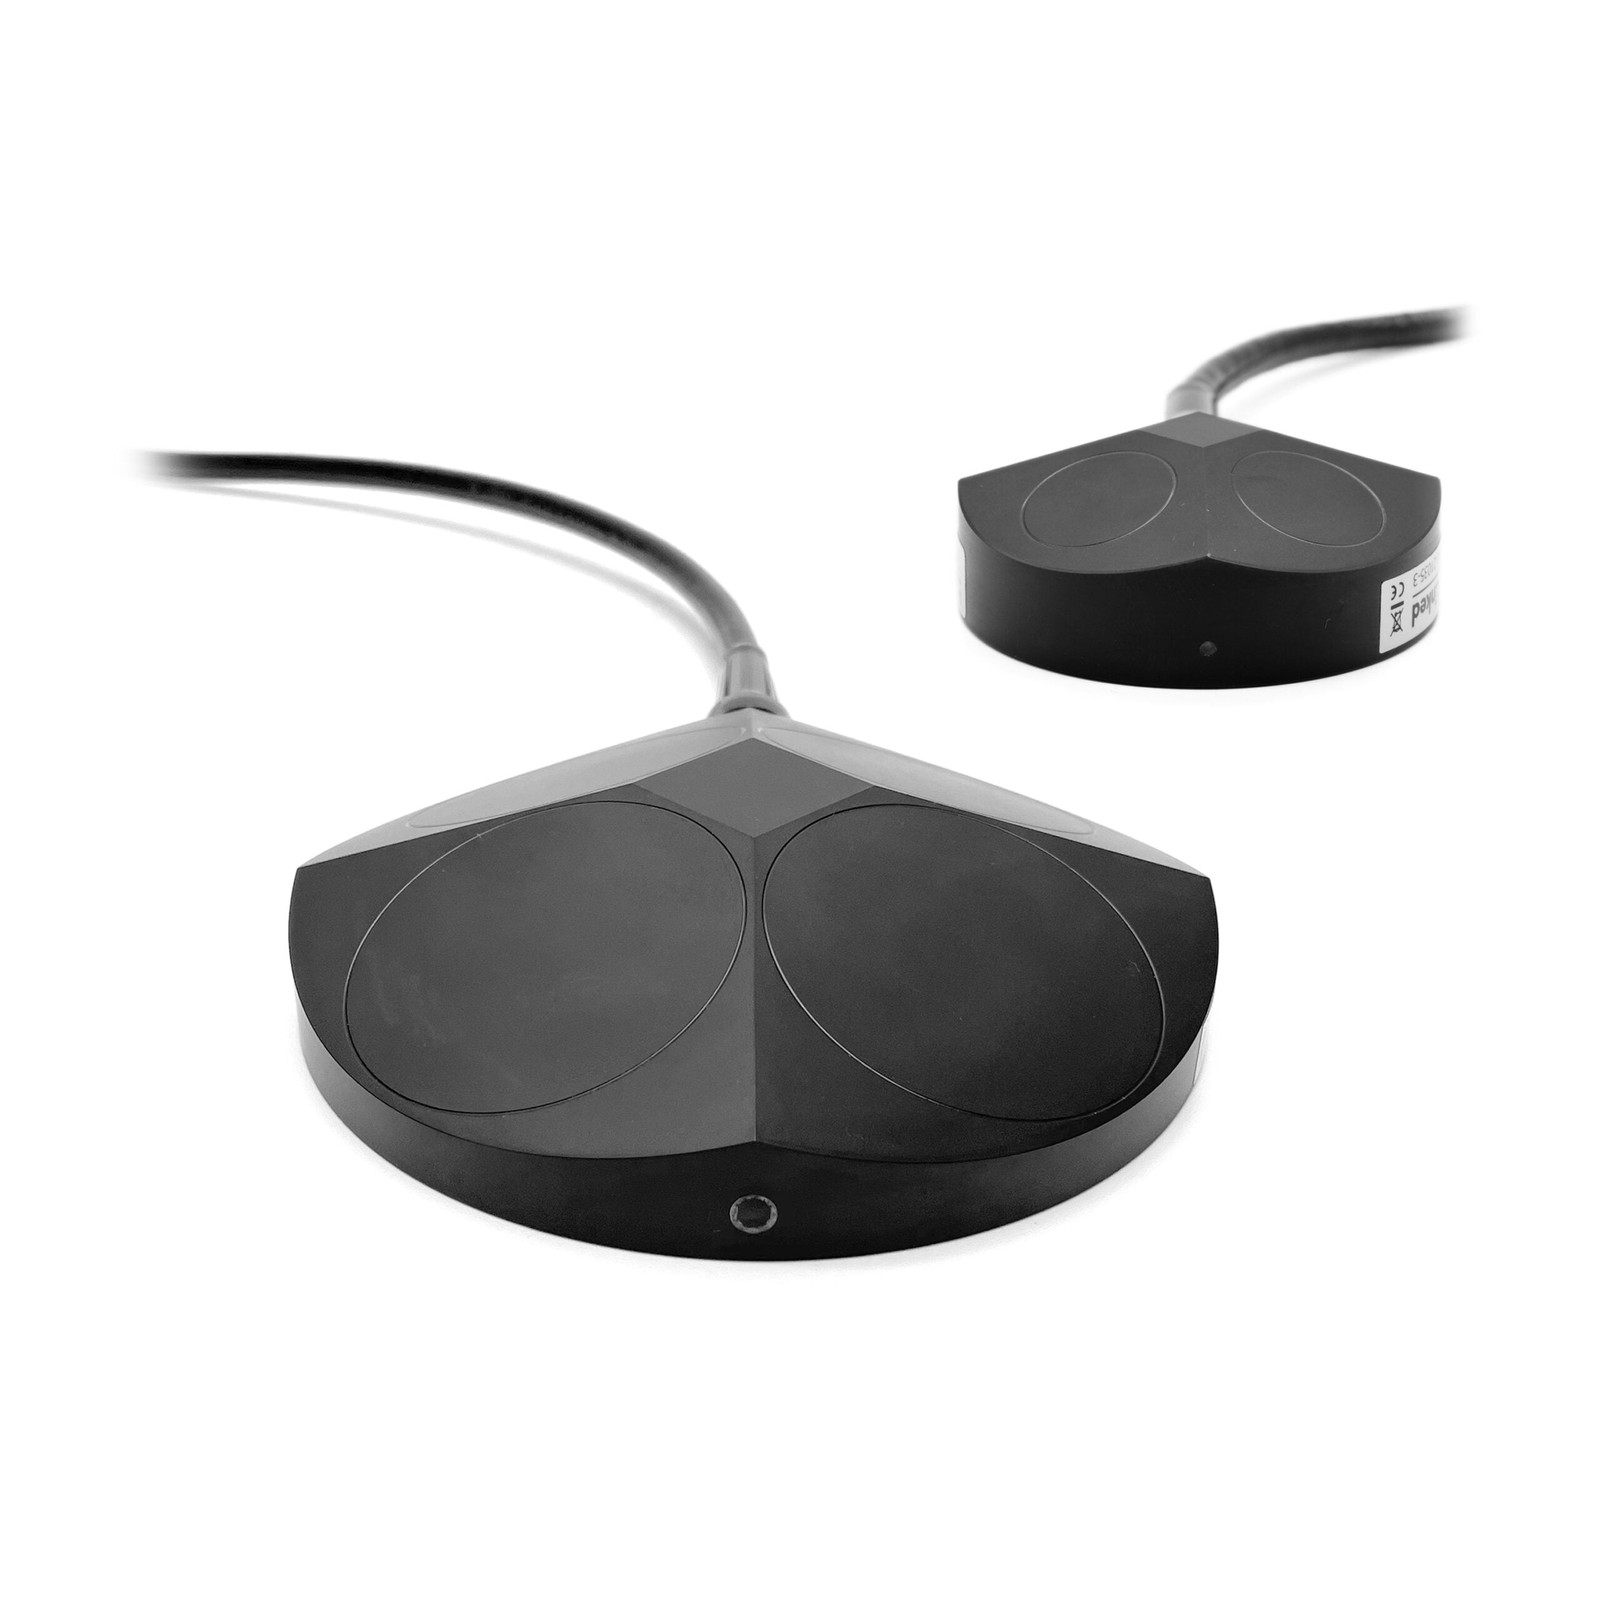
\includegraphics[height=2.3cm, keepaspectratio]{dvl_a50.jpg}\\
        \vspace{0.2em}
        \footnotesize\textbf{Capteur DVL-A50}\\
        \scriptsize\textit{Transducteur 4 faisceaux Janus 1 MHz}
      \end{center}
      \begin{center}
        \begin{tikzpicture}[scale=0.72]
          \draw[thick, fill=OceanMedium!20, rounded corners] (-1.8, 0.8) rectangle (1.8, 1.3);
          \node at (0, 1.05) {\tiny Châssis BlueROV2};
          \draw[thick, fill=black!80] (-0.7, 0.3) rectangle (0.7, 0.8);
          \node[white] at (0, 0.55) {\tiny DVL};
          \draw[->, line width=1.2pt, OceanCyan] (-0.5, 0.3) -- (-1.5, -0.8);
          \draw[->, line width=1.2pt, OceanCyan] (0.5, 0.3) -- (1.5, -0.8);
          \draw[->, line width=1.2pt, OceanMedium] (-0.2, 0.3) -- (-0.6, -0.8);
          \draw[->, line width=1.2pt, OceanMedium] (0.2, 0.3) -- (0.6, -0.8);
          \draw[thick, fill=brown!30] (-2, -0.8) rectangle (2, -1.05);
          \node at (0, -0.92) {\tiny Fond marin (Bottom-Track)};
        \end{tikzpicture}
      \end{center}
    \end{column}
  \end{columns}
\end{frame}

\begin{frame}{4.3 Intégration d'un Capteur Scientifique Tiers}
  \begin{columns}[T]
    \begin{column}{0.49\textwidth}
      \begin{block}{\tech{1. Intégration Mécanique \& Câblage}}
        \scriptsize
        \begin{itemize}
          \item Traversée du caisson : Penetrateur \tech{WetLink M10} ou connecteur débrochable (\tech{Cobalt} / \tech{SubConn}).
          \item Raccordement interne sur le \textbf{Raspberry Pi} :
            \begin{itemize}\tiny
              \item Port USB via convertisseur série RS-232 / RS-485 isolé.
              \item Bus I2C / SPI / ADC sur la carte Navigator.
            \end{itemize}
        \end{itemize}
      \end{block}
    \end{column}

    \begin{column}{0.49\textwidth}
      \begin{block}{\succw{2. Flux Logiciel sous BlueOS}}
        \scriptsize
        \begin{itemize}
          \item Démon Python lisant les trames du capteur (température, DO, turbidité).
          \item \succw{Temps réel surface} : envoi MAVLink \code{NAMED\_VALUE\_FLOAT} pour affichage dans \textbf{Cockpit}.
          \item \succw{Post-mission} : CSV local ou topics \textbf{ROS 2} enregistrés en \code{rosbag2}.
        \end{itemize}
      \end{block}
    \end{column}
  \end{columns}
\end{frame}

\begin{frame}{4.4 Le C{\oe}ur Océanographique : La Mesure CTD}
  \begin{columns}[c]
    \begin{column}{0.55\textwidth}
      \textbf{CTD : \textit{Conductivity - Temperature - Depth}}
      \begin{itemize}
        \item \textbf{Conductivité} : cellule inductive ou à électrodes.
        \item \textbf{Température} : thermistance étalonnée (précision $<0.01^\circ\text{C}$).
        \item \textbf{Pression} : assurée directement par le capteur \tech{Bar30} !
      \end{itemize}

      \vspace{0.4em}
      \begin{block}{Paramètres Dérivés Fondamentaux (TEOS-10)}
        \begin{itemize}
          \item \textbf{Salinité absolue} $S_A$ ($\text{g/kg}$ ou PSU).
          \item \textbf{Masse volumique} $\rho(S, T, P)$.
          \item \tech{Célérité du son} $c(S, T, P)$ : \textbf{indispensable} pour corriger la portée des sonars et de l'USBL !
        \end{itemize}
      \end{block}
    \end{column}

    \begin{column}{0.45\textwidth}
      \begin{center}
        \begin{tikzpicture}[scale=0.85]
          \draw[->] (0,0) -- (3.5,0) node[right] {\small $T, S, \rho$};
          \draw[->] (0,0) -- (0,-3.5) node[below] {\small Profondeur $z$};
          
          \draw[thick, OceanCoral] (3, 0) -- (3, -0.8) to[out=-90, in=90] (0.8, -2.2) -- (0.7, -3.4) node[right] {\small $T^\circ\text{C}$};
          \node[OceanCoral, right] at (1.8,-1.5) {\footnotesize Thermocline};
          
          \draw[thick, OceanCyan] (0.8, 0) -- (0.8, -0.8) to[out=-90, in=90] (2.8, -2.2) -- (2.9, -3.4) node[right] {\small $\rho$};
          \node[OceanCyan, left] at (2.2,-1.5) {\footnotesize Pycnocline};
        \end{tikzpicture}
      \end{center}
      \small
      Le gradient de célérité du son $c(z)$ réfracte les ondes acoustiques.
    \end{column}
  \end{columns}
\end{frame}

\begin{frame}{4.5 Photogrammétrie Benthique avec BlueROV2}
  \begin{columns}[T]
    \begin{column}{0.52\textwidth}
      \textbf{Équipement requis pour le relevé 3D} :
      \begin{itemize}
        \item \textbf{Caméra HD Low-Light} intégrée ou caméra reflex/action cam (GoPro / Sony RX0) dans un caisson dédié.
        \item \textbf{Projecteurs Lumen (BlueRobotics)} : $2 \times 1500\,\text{lumens}$ ou plus, montés aux extrémités du châssis (pour limiter la rétrodiffusion de la neige marine).
        \item Contrôle de l'altitude via le Ping Sonar ou DVL ($1.5\text{--}2.0\,\text{m}$ du fond).
        \item Recouvrement inter-images $>75\%$ en marche avant.
      \end{itemize}
    \end{column}

    \begin{column}{0.48\textwidth}
      \begin{block}{Chaîne de Traitement 3D}
        \begin{itemize}
          \item Extraction des images et synchronisation avec la trajectoire DVL/USBL.
          \item Logiciels SfM : \textbf{Agisoft Metashape}, \textbf{Meshroom} ou \textbf{CloudCompare}.
          \item Correction de la distorsion optique induite par le dôme acrylique.
          \item \succw{Résultat} : orthomosaïque géoréférencée centimétrique et modèle numérique d'élévation (MNE) 3D d'herbiers ou de récifs.
        \end{itemize}
      \end{block}
    \end{column}
  \end{columns}
\end{frame}

\begin{frame}{4.6 Du Signal Brut au Format Standard Océano : NetCDF \& GeoTIFF}
  \begin{center}
    \begin{tikzpicture}[scale=0.85, auto, node distance=1.3cm, >=Latex]
      \node[draw=OceanDeep, fill=OceanDeep!10, rounded corners, rectangle, minimum width=2.6cm, align=center] (raw_nav) {
        \textbf{Navigation}\\
        \footnotesize IMU + DVL + Bar30
      };
      \node[draw=OceanCoral, fill=OceanCoral!10, rounded corners, rectangle, minimum width=2.6cm, align=center, below=0.7cm of raw_nav] (usbl) {
        \textbf{Fixes Acoustiques}\\
        \footnotesize USBL surface + GNSS
      };
      \node[draw=OceanMedium, fill=OceanMedium!20, rounded corners, rectangle, minimum width=3.2cm, align=center, right=1.2cm of raw_nav] (smooth) {
        \textbf{Fusion \& Interpolation}\\
        \footnotesize Trajectoire 4D $(x,y,z,t)$
      };
      \node[draw=OceanGreen, fill=OceanGreen!10, rounded corners, rectangle, minimum width=2.6cm, align=center, above=0.7cm of smooth] (sensors) {
        \textbf{Mesures Capteurs}\\
        \footnotesize CTD, Fluorimètre, Sonar
      };
      \node[draw=OceanCyan, fill=OceanCyan!20, line width=1.5pt, rounded corners, rectangle, minimum width=3.2cm, align=center, right=1.2cm of smooth] (data_product) {
        \textbf{Produit FAIR Final}\\
        \footnotesize \textbf{NetCDF-4} (CF Metadata)\\
        \footnotesize GeoTIFF, Nuage LAS
      };

      \draw[->, thick, OceanDeep] (raw_nav) -- (smooth);
      \draw[->, thick, OceanCoral] (usbl) -| (smooth);
      \draw[->, thick, OceanGreen] (sensors) -- (smooth);
      \draw[->, line width=1.5pt, OceanCyan] (smooth) -- (data_product);
    \end{tikzpicture}
  \end{center}

  \begin{block}{Les Bonnes Pratiques FAIR (Findable, Accessible, Interoperable, Reusable)}
    \begin{itemize}
      \item Enregistrer les métadonnées dès l'acquisition (identifiant du vecteur, étalonnage de la sonde, opérateur).
      \item Utiliser les conventions CF (\textit{Climate and Forecast}) pour que vos données soient directement lisibles par les outils d'analyse (Python \code{xarray}, Ocean Data View, QGIS).
    \end{itemize}
  \end{block}
\end{frame}
